\chapter{Diagram Biner Cair--Uap dan Distilasi}\label{ch:b2:liquid-vapour-diagrams}

Sebuah alat suling tembaga mengubah anggur yang kadar alkoholnya hanya
beberapa persen menjadi minuman keras yang berlipat-lipat lebih kuat;
kolom kilang memecah minyak mentah menjadi fraksi-fraksinya, dari gas
sampai bahan bakar berat. Keduanya bertumpu pada satu fakta: uap di atas
campuran yang mendidih lebih kaya akan komponen yang lebih mudah menguap
daripada cairannya. Ulangi penguapan dan pengembunan itu cukup banyak
kali, dan pemisahannya menjadi setajam yang dikehendaki --- dengan satu
pengecualian: tidak ada distilasi, sepanjang apa pun kolomnya, yang
membawa etanol melampaui sekitar 95 persen massa. Bab ini menggambar
diagram-diagram yang menyatakan bagaimana campuran dua cairan mendidih,
lalu memakainya untuk merancang kolom dan melihat di mana kolom itu harus
berhenti.

\begin{recall}
\Cref{ch:b2:chemical-potential}: \omterm{def:b2:chemical-potential:chemical-potential}{potensial kimia}, \omterm{thm:b2:chemical-potential:raoult}{hukum Raoult} dan \omterm{def:b2:chemical-potential:ideal-mixture}{campuran
ideal}, \omterm{def:b2:chemical-potential:activity-coefficient}{koefisien aktivitas} dan simpangan dari \omterm{thm:b2:chemical-potential:raoult}{hukum Raoult}, hubungan
Gibbs--Duhem. \Cref{ch:b2:equilibrium-shifts}: \omterm{def:b2:equilibrium-shifts:variance}{varians}. Jilid Tahun 1,
tentang teknik laboratorium: distilasi sederhana, cairan yang dapat
bercampur dan yang tidak dapat bercampur. Jilid sekolah: distilasi dan
hidrodistilasi.
\end{recall}

\begin{omfigure}
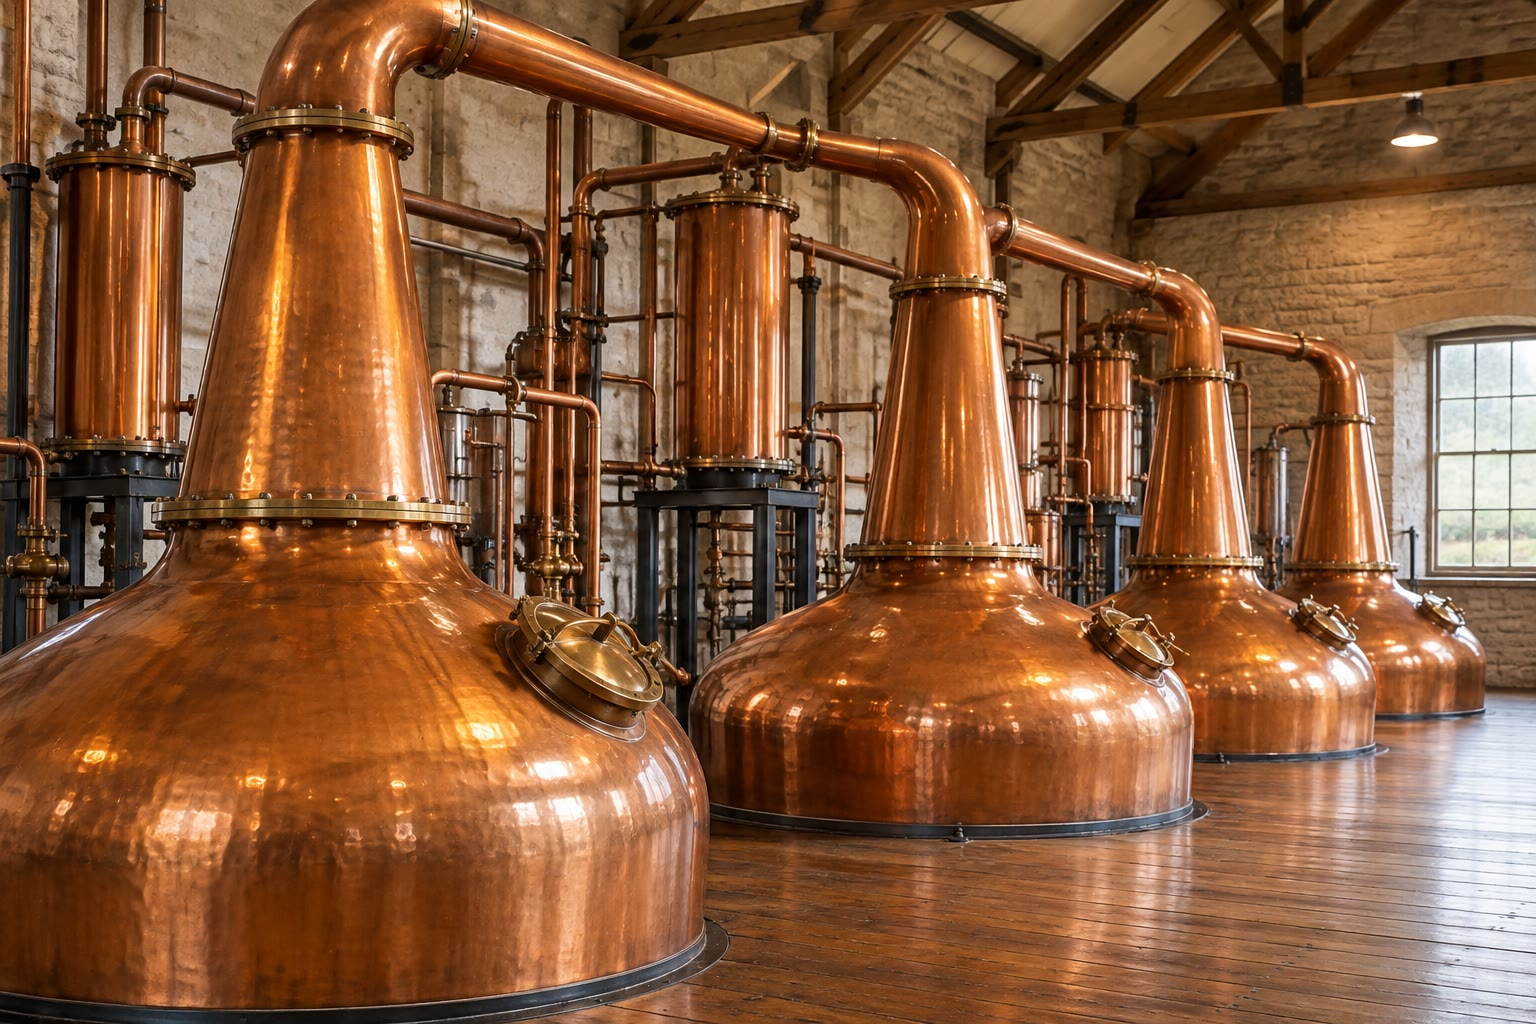
\includegraphics[width=0.62\linewidth]{images/book3/ai/b2-07-pot-stills.jpg}

{\small Alat suling tembaga di sebuah penyulingan. Setiap muatan cairan
fermentasi didihkan dan uapnya diembunkan: distilat pertama beberapa kali
lebih kaya etanol daripada cairan fermentasinya, dan distilasi kedua
memekatkannya lebih lanjut.}
\end{omfigure}

\section{Campuran ideal}

Dalam bab ini kedua cairan diberi nomor 1 (yang lebih mudah menguap,
dengan titik didih lebih rendah) dan 2; $x$ adalah fraksi mol 1 dalam
cairan, $y$ fraksi molnya dalam uap, yang dianggap sebagai gas ideal.

\begin{definition}[Diagram biner]\label{def:b2:liquid-vapour-diagrams:binary-diagram}
Yang disebut \emph{diagram biner}\index{diagram biner} adalah diagram yang
menunjukkan, untuk campuran dua komponen, fase-fase mana yang ada dan
dengan komposisi berapa, sebagai fungsi komposisi keseluruhan dan satu
variabel lain. Sebuah \emph{diagram isobarik}\index{diagram isobarik}
digambar pada bidang (komposisi, suhu) pada tekanan tetap; sebuah
\emph{diagram isotermal}\index{diagram isotermal} pada bidang (komposisi,
tekanan) pada suhu tetap.
\end{definition}

\begin{definition}[Kurva gelembung dan kurva embun]\label{def:b2:liquid-vapour-diagrams:bubble-dew}
Pada diagram cair--uap, \emph{kurva gelembung}\index{kurva gelembung}
memberikan komposisi cairan yang berada dalam kesetimbangan dengan uap,
sedangkan \emph{kurva embun}\index{kurva embun} memberikan komposisi uap
yang berada dalam kesetimbangan dengan cairan. Untuk campuran dengan
komposisi tertentu pada tekanan tetap, \emph{titik gelembung}\index{titik gelembung}
adalah suhu ketika gelembung uap pertama muncul pada pemanasan, dan
\emph{titik embun}\index{titik embun} adalah suhu ketika tetes cairan
pertama muncul pada pendinginan uap.
\end{definition}

\begin{proposition}[Kurva ideal]\label{prop:b2:liquid-vapour-diagrams:ideal-curves}
Untuk \omterm{def:b2:chemical-potential:ideal-mixture}{campuran ideal} pada suhu $T$, dengan $p_1^*$ dan $p_2^*$ tekanan uap
cairan-cairan murninya, \omterm{def:b2:liquid-vapour-diagrams:bubble-dew}{kurva gelembung} \omterm{def:b2:liquid-vapour-diagrams:binary-diagram}{diagram isotermal} adalah garis
lurus $p = p_2^* + x(p_1^* - p_2^*)$, dan \omterm{def:b2:liquid-vapour-diagrams:bubble-dew}{kurva embunnya} adalah hiperbola
\[
  p = \frac{1}{y/p_1^* + (1 - y)/p_2^*} .
\]
\end{proposition}

\begin{proof}
\omterm{thm:b2:chemical-potential:raoult}{Hukum Raoult} memberikan tekanan parsial $p_1 = xp_1^*$ dan
$p_2 = (1 -
x)p_2^*$; jumlahnya adalah tekanan total, yang linear dalam
$x$. Dalam uap, $y = p_1/p$, sehingga $x = yp/p_1^*$ dan
$1 - x = (1 - y)p/p_2^*$; dengan menjumlahkannya,
$1 = p\,[y/p_1^* + (1 - y)/p_2^*]$.
\end{proof}

\begin{proposition}[Uap lebih kaya akan komponen yang lebih mudah menguap]\label{prop:b2:liquid-vapour-diagrams:richer}
Untuk \omterm{def:b2:chemical-potential:ideal-mixture}{campuran ideal} dengan $p_1^* > p_2^*$ dan $0 < x < 1$, $y > x$.
\end{proposition}

\begin{proof}
$y = xp_1^*/p$ dengan $p = xp_1^* + (1 - x)p_2^* < p_1^*$ karena $p$ adalah
rata-rata berbobot $p_1^*$ dan $p_2^*$, yang terletak tegas di antara
keduanya. Jadi $y >
x$.
\end{proof}

Diagram isobariklah yang memerikan distilasi, yang berlangsung pada tekanan
atmosfer. Diagram ini tidak mempunyai rumus sederhana: untuk setiap suhu
di antara kedua titik didih, $p_1^*(T)$ dan $p_2^*(T)$ dihitung (di sini
dengan persamaan Antoine, $\log_{10}(p^*/\unit{bar}) = A - B/(T + C)$, yang
dicocokkan dengan tekanan uap terukur), lalu komposisi cairan dan uap yang
memberikan tekanan total \qty{1.013}{bar}:
\[
  x = \frac{p - p_2^*(T)}{p_1^*(T) - p_2^*(T)}, \qquad y = \frac{x\,p_1^*(T)}{p} .
\]
\omterm{def:b2:liquid-vapour-diagrams:bubble-dew}{Kurva gelembung} tidak lagi lurus; \omterm{def:b2:liquid-vapour-diagrams:bubble-dew}{kurva embun} tetap berada di atasnya,
dan uap tetap lebih kaya akan komponen yang ringan.

\begin{example}[Benzena dan toluena pada \qty{90}{\degreeCelsius}]\label{ex:b2:liquid-vapour-diagrams:benzene-toluene}
Benzena dan toluena membentuk campuran yang hampir ideal. Pada
\qty{90}{\degreeCelsius}, persamaan Antoine memberikan
$p_1^* = \qty{1.361}{bar}$ (benzena) dan $p_2^* =
\qty{0.542}{bar}$
(toluena). Pada \qty{1.013}{bar}: $x = (1.013 - 0.542)/(1.361 -
0.542) = 0.575$ dan $y = 0.575 \times 1.361/1.013 = 0.773$. Cairan dengan
57.5~\% benzena (dalam mol) mendidih pada \qty{90}{\degreeCelsius} dan
menghasilkan uap dengan 77~\%.
% ledger: antoine:benzene.A, antoine:benzene.B, antoine:benzene.C, antoine:toluene.A, antoine:toluene.B, antoine:toluene.C
\end{example}

\begin{omfigure}
\begin{tikzpicture}
\begin{axis}[omphase, width=0.47\linewidth, height=6cm, ymin=78, ymax=113,
  xlabel={$x$, $y$ (benzena)}, ylabel={$T$ (\unit{\degreeCelsius})},
  title={\small isobarik, \qty{1.013}{bar}}]
\addplot[omliquidus] table[x=x, y=T] {figdata/out/bachelor-2-liquid-vapour-a.dat};
\addplot[omsolidus] table[x=y, y=T] {figdata/out/bachelor-2-liquid-vapour-a.dat};
\draw[tieline] (axis cs:0.405,95) -- (axis cs:0.626,95);
\fill (axis cs:0.5,95) circle (1.3pt);
\draw[->, thick] (axis cs:0.5,82) -- (axis cs:0.5,104) node[above, font=\scriptsize] {pemanasan};
\node[font=\scriptsize] at (axis cs:0.2,85) {cair};
\node[font=\scriptsize] at (axis cs:0.85,108) {uap};
\node[font=\scriptsize, omDef, anchor=north] at (axis cs:0.22,96) {gelembung};
\node[font=\scriptsize, omThm, anchor=south west] at (axis cs:0.62,101) {embun};
\end{axis}
\end{tikzpicture}\hfill
\begin{tikzpicture}
\begin{axis}[omphase, width=0.47\linewidth, height=6cm, ymin=0.3, ymax=1.1,
  xlabel={$x$, $y$ (benzena)}, ylabel={$p$ (\unit{bar})},
  title={\small isotermal, \qty{80}{\degreeCelsius}}]
\addplot[omliquidus] table[x=x, y=pbub] {figdata/out/bachelor-2-liquid-vapour-b.dat};
\addplot[omsolidus] table[x=x, y=pdew] {figdata/out/bachelor-2-liquid-vapour-b.dat};
\node[font=\scriptsize] at (axis cs:0.75,0.98) {cair};
\node[font=\scriptsize] at (axis cs:0.2,0.36) {uap};
\end{axis}
\end{tikzpicture}

{\small Benzena--toluena, dihitung dari \omterm{thm:b2:chemical-potential:raoult}{hukum Raoult} dan persamaan
Antoine. Kiri, pada tekanan atmosfer: \omterm{def:b2:liquid-vapour-diagrams:bubble-dew}{kurva gelembung} (biru) dan \omterm{def:b2:liquid-vapour-diagrams:bubble-dew}{kurva
embun} (merah); cairan dengan komposisi 0.5 mulai mendidih pada
\qty{92.1}{\degreeCelsius} dan seluruhnya menjadi uap pada
\qty{98.8}{\degreeCelsius}; pada \qty{95}{\degreeCelsius} (garis hubung
putus-putus) campuran itu terbagi menjadi cairan 0.405 dan uap 0.626.
Kanan, pada \qty{80}{\degreeCelsius}: \omterm{def:b2:liquid-vapour-diagrams:bubble-dew}{kurva gelembung} lurus, \omterm{def:b2:liquid-vapour-diagrams:bubble-dew}{kurva embun}
berupa hiperbola, dan cairan kini berada di atas.}
% ledger: antoine:benzene.A, antoine:toluene.A (all six parameters in figdata/bachelor-2/liquid-vapour.py)
\end{omfigure}

\section{Membaca diagram}

\begin{proposition}[Varians campuran biner dua fase]\label{prop:b2:liquid-vapour-diagrams:variance}
Campuran dua komponen dalam dua fase mempunyai \omterm{def:b2:equilibrium-shifts:variance}{varians} 2. Pada tekanan
tetap, suhu saja sudah menetapkan komposisi kedua fase: komposisi itu
dibaca pada kedua ujung ruas mendatar yang melalui titik representatif,
yang disebut garis hubung.
\end{proposition}

\begin{proof}
Variabel intensif: $T$, $p$, $x$, $y$. Hubungan: kesamaan \omterm{def:b2:chemical-potential:chemical-potential}{potensial kimia}
1 dan 2 di antara fase-fase. $v = 4 - 2 = 2$ (aturan fase
$v = n - r + 2 - \varphi$ memberikan hasil yang sama dengan $n = 2$,
$r = 0$, $\varphi = 2$). Menetapkan $p$ menyisakan satu derajat
kebebasan: $x(T)$ dan $y(T)$ adalah kedua kurva itu.
\end{proof}

\begin{theorem}[Aturan tuas]\label{thm:b2:liquid-vapour-diagrams:lever}
Campuran dengan komposisi keseluruhan $z$, yang terbagi menjadi cairan
dengan komposisi $x$ dan uap dengan komposisi $y$, mengandung jumlah zat
$n_L$ cairan dan $n_V$ uap sedemikian rupa sehingga
\[
  n_L\,(z - x) = n_V\,(y - z), \qquad \frac{n_V}{n_L + n_V} = \frac{z - x}{y - x} .
\]
Inilah \emph{aturan tuas}\index{aturan tuas}: setiap fase makin melimpah
makin dekat komposisinya dengan komposisi keseluruhan, seperti beban pada
tuas yang bertumpu di $z$.
\end{theorem}

\begin{proof}
Kekekalan komponen 1: $(n_L + n_V)z = n_Lx + n_Vy$, sehingga
$n_L(z - x) =
n_V(y - z)$; bagilah dengan $n_L + n_V$ lalu susun ulang.
\end{proof}

\omterm{thm:b2:liquid-vapour-diagrams:lever}{Aturan tuas} berlaku dengan fraksi mol dan jumlah zat, seperti di sini,
atau dengan fraksi massa dan massa: kekekalan yang dipakai sama.

\begin{method}[Membaca diagram biner]\label{met:b2:liquid-vapour-diagrams:read-diagram}
\begin{enumerate}
  \item Letakkan titik (komposisi keseluruhan, suhu) dan sebutkan daerahnya:
        cair, uap, atau cair + uap.
  \item Dalam daerah dua fase, tariklah garis hubung melalui titik itu;
        kedua ujungnya memberikan komposisi cairan (pada \omterm{def:b2:liquid-vapour-diagrams:bubble-dew}{kurva gelembung})
        dan komposisi uap (pada \omterm{def:b2:liquid-vapour-diagrams:bubble-dew}{kurva embun}).
  \item Tentukan proporsi fase-fasenya dengan \omterm{thm:b2:liquid-vapour-diagrams:lever}{aturan tuas}.
  \item Untuk mengikuti pemanasan, geserlah titik itu ke atas: gelembung
        pertama muncul pada \omterm{def:b2:liquid-vapour-diagrams:bubble-dew}{kurva gelembung}, tetes terakhir lenyap pada
        \omterm{def:b2:liquid-vapour-diagrams:bubble-dew}{kurva embun}; di antara keduanya, cairan makin miskin akan komponen
        yang ringan.
\end{enumerate}
\end{method}

\begin{example}[Penguapan kilat pada \qty{95}{\degreeCelsius}]\label{ex:b2:liquid-vapour-diagrams:flash}
Sebanyak \qty{100}{mol} campuran ekuimolar benzena--toluena dibawa ke
\qty{95}{\degreeCelsius} pada tekanan atmosfer. Garis hubung memberikan
$x =
0.405$, $y = 0.626$; fraksi uapnya
$(0.500 - 0.405)/(0.626 - 0.405) =
0.43$: \qty{43}{mol} uap yang
mengandung $43 \times 0.626 = \qty{27}{mol}$ benzena, dan \qty{57}{mol}
cairan yang mengandung \qty{23}{mol}. Satu tahap kesetimbangan memang
memperkaya, tetapi hanya sedikit.
\end{example}

\section{Campuran nyata dan azeotrop}

Jika \omterm{def:b2:chemical-potential:activity-coefficient}{koefisien aktivitas} berbeda dari 1 (\cref{ch:b2:chemical-potential}),
tekanan parsial menyimpang dari garis-garis lurus Raoult. Dengan simpangan
positif ($\gamma > 1$: molekul tak sejenis saling menarik lebih lemah
daripada molekul sejenis), tekanan total terletak di atas garis ideal;
dengan simpangan negatif, di bawahnya. Jika simpangannya cukup kuat,
tekanan total melewati sebuah ekstremum.

\begin{definition}[Azeotrop]\label{def:b2:liquid-vapour-diagrams:azeotrope}
Yang disebut \emph{azeotrop}\index{azeotrop} adalah campuran cair yang
mendidih tanpa berubah komposisi: uap yang dihasilkannya mempunyai
komposisi yang sama dengan komposisinya sendiri. Sebuah \emph{azeotrop
positif}\index{azeotrop positif} (simpangan positif) mempunyai maksimum
tekanan pada \omterm{def:b2:liquid-vapour-diagrams:binary-diagram}{diagram isotermal} dan minimum suhu didih pada \omterm{def:b2:liquid-vapour-diagrams:binary-diagram}{diagram
isobarik}; sebuah \emph{azeotrop negatif}\index{azeotrop negatif}
sebaliknya.
\end{definition}

\begin{theorem}[Teorema Gibbs--Konovalov]\label{thm:b2:liquid-vapour-diagrams:konovalov}
Pada \omterm{def:b2:liquid-vapour-diagrams:binary-diagram}{diagram biner} cair--uap, pada ekstremum tekanan total (pada suhu
tetap) atau suhu didih (pada tekanan tetap), cairan dan uap mempunyai
komposisi yang sama. Sebaliknya, di tempat kedua komposisi itu sama,
kurva-kurvanya mempunyai garis singgung mendatar yang sama.
\end{theorem}

\begin{proof}[Bukti pada suhu tetap]
Hubungan Gibbs--Duhem untuk cairan pada $T$ tetap (dengan mengabaikan
pengaruh kecil $p$ pada cairan) adalah $x\,d\mu_1 + (1 - x)\,d\mu_2 = 0$.
Pada kesetimbangan $\mu_i = \mu_i^\circ + RT\ln(p_i/p^\circ)$ dengan
$p_1 = yp$, $p_2 = (1 - y)p$, sehingga
\[
  x\,d\ln(yp) + (1 - x)\,d\ln((1 - y)p) = 0
  \quad\Longrightarrow\quad
  d\ln p = -\Big(\frac{x}{y} - \frac{1 - x}{1 - y}\Big)dy
  = \frac{y - x}{y(1 - y)}\,dy .
\]
Karena $y$ bertambah seiring $x$ (jika tidak, cairan itu tidak stabil),
$dp/dx = 0$ tepat di tempat $y = x$. Kasus isobarik diperoleh dari
perhitungan serupa yang memperhitungkan kebergantungan $\mu_i^\circ$ pada
suhu; perhitungan itu tidak dilakukan di sini.
\end{proof}

Rumus itu menyatakan lebih banyak lagi: di tempat $y > x$, tekanan
bertambah seiring $x$ --- menambahkan komponen yang diperkaya di dalam uap
membuat cairan lebih mudah menguap, dan inilah hukum pertama Konovalov.

\begin{example}[Etanol dan air]\label{ex:b2:liquid-vapour-diagrams:ethanol-water}
Etanol dan air menyimpang secara positif dari \omterm{thm:b2:chemical-potential:raoult}{hukum Raoult} dan membentuk
\omterm{def:b2:liquid-vapour-diagrams:azeotrope}{azeotrop} dengan 95~\% massa etanol pada tekanan atmosfer. Dengan
$M = 46.07$ dan \qty{18.02}{g/mol}, fraksi mol etanolnya adalah
\[
  x_{\text{az}} = \frac{95/46.07}{95/46.07 + 5/18.02} = 0.881 .
\]
\omterm{def:b2:liquid-vapour-diagrams:azeotrope}{Azeotrop} itu mendidih sedikit di bawah etanol murni
(\qty{78.3}{\degreeCelsius}). Diagram di bawah dihitung dari model
aktivitas satu parameter, $\ln\gamma_1 = A(1 -
x)^2$, $\ln\gamma_2 = Ax^2$,
yang parameternya ($A = 1.09$) dicocokkan agar \omterm{def:b2:liquid-vapour-diagrams:azeotrope}{azeotrop} jatuh pada
komposisi itu: model ini mereproduksi bentuknya, dan menempatkan \omterm{def:b2:liquid-vapour-diagrams:azeotrope}{azeotrop}
pada \qty{77.9}{\degreeCelsius}.
% ledger: azeo:ethanol-water.w, aw:C, aw:H, aw:O, antoine:ethanol.A, antoine:ethanol.B, antoine:ethanol.C, antoine:water.A, antoine:water.B, antoine:water.C
\end{example}

\begin{omfigure}
\begin{tikzpicture}
\begin{axis}[omphase, width=0.47\linewidth, height=6cm, ymin=76, ymax=101,
  xlabel={$x$, $y$ (etanol)}, ylabel={$T$ (\unit{\degreeCelsius})},
  title={\small etanol--air (model)}]
\addplot[omliquidus] table[x=x, y=T] {figdata/out/bachelor-2-liquid-vapour-c.dat};
\addplot[omsolidus] table[x=y, y=T] {figdata/out/bachelor-2-liquid-vapour-c.dat};
\fill (axis cs:0.881,77.92) circle (1.5pt);
\draw[densely dotted] (axis cs:0.881,77.92) -- (axis cs:0.881,76);
\node[font=\scriptsize, anchor=south] at (axis cs:0.80,80.5) {azeotrop};
\draw[thin] (axis cs:0.80,80.5) -- (axis cs:0.875,78.2);
\node[font=\scriptsize] at (axis cs:0.25,79.5) {cair};
\node[font=\scriptsize] at (axis cs:0.5,95) {uap};
\end{axis}
\end{tikzpicture}\hfill
\begin{tikzpicture}
\begin{axis}[omphase, width=0.47\linewidth, height=6cm, ymin=78, ymax=120,
  xlabel={$x$, $y$ (komponen 1)}, ylabel={$T$ (\unit{\degreeCelsius})},
  title={\small simpangan negatif (model)}]
\addplot[omliquidus] table[x=x, y=T] {figdata/out/bachelor-2-liquid-vapour-d.dat};
\addplot[omsolidus] table[x=y, y=T] {figdata/out/bachelor-2-liquid-vapour-d.dat};
\fill (axis cs:0.29,116.7) circle (1.5pt);
\node[font=\scriptsize, anchor=west] at (axis cs:0.33,118) {azeotrop};
\node[font=\scriptsize] at (axis cs:0.6,85) {cair};
\node[font=\scriptsize] at (axis cs:0.75,116) {uap};
\end{axis}
\end{tikzpicture}

{\small Kiri: etanol--air pada tekanan atmosfer, dari model satu parameter
yang dicocokkan dengan komposisi \omterm{def:b2:liquid-vapour-diagrams:azeotrope}{azeotrop} (0.881); \omterm{def:b2:liquid-vapour-diagrams:azeotrope}{azeotrop} itu mendidih
di bawah kedua cairan murni. Kanan: pasangan model dengan simpangan
negatif yang kuat ($A = -2.0$, tekanan uap benzena dan toluena);
\omterm{def:b2:liquid-vapour-diagrams:azeotrope}{azeotropnya} mendidih di atas keduanya.}
% ledger: azeo:ethanol-water.w, antoine:ethanol.A, antoine:water.A (model in figdata/bachelor-2/liquid-vapour.py)
\end{omfigure}

\section{Distilasi fraksional}

\begin{definition}[Distilasi fraksional]\label{def:b2:liquid-vapour-diagrams:fractional-distillation}
Yang disebut \emph{distilasi fraksional}\index{distilasi fraksional}
memisahkan komponen-komponen campuran cair di dalam kolom tempat uap yang
naik dan cairan yang turun dipertemukan berulang-ulang. Sebuah
\emph{pelat teoretis}\index{pelat teoretis} adalah tahap kolom yang uap
dan cairan keluarannya berada dalam kesetimbangan satu sama lain.
Selanjutnya, \emph{rasio refluks}\index{rasio refluks} adalah rasio
jumlah kondensat yang dikembalikan ke puncak kolom terhadap jumlah yang
diambil sebagai distilat.
\end{definition}

Pada setiap pelat, uap dari bawah menggelegak melewati cairan dari atas;
uap itu keluar lebih kaya akan komponen yang ringan, cairannya lebih
miskin. Di puncak, uap diembunkan, sebagian dikembalikan sebagai refluks,
sisanya diambil sebagai distilat; di dasar, sebuah pendidih ulang
mendidihkan sebagian cairan. Pada \textit{refluks total} tidak ada yang
diambil: kolom bekerja paling baik, dan uap yang meninggalkan sebuah pelat
mempunyai komposisi cairan yang turun ke atasnya.


Untuk pasangan ideal, \textit{volatilitas relatif} $\alpha = p_1^*/p_2^*$
hanya sedikit berubah di sepanjang kolom: dari 2.60 pada titik didih
benzena sampai 2.35 pada titik didih toluena. Pada setiap \omterm{def:b2:liquid-vapour-diagrams:fractional-distillation}{pelat teoretis}
\[
  \frac{y}{1 - y} = \frac{xp_1^*}{(1 - x)p_2^*} = \alpha\,\frac{x}{1 - x} .
\]

\begin{omfigure}
\begin{minipage}[b]{0.58\linewidth}\centering
\begin{tikzpicture}[font=\small, >={Stealth}, scale=0.8, every node/.style={transform shape}]
  \draw[thick, fill=gray!8] (0,0) rectangle (1.8,7);
  \foreach \k in {1,...,6} {
    \pgfmathsetmacro{\yy}{\k}
    \ifodd\k
      \draw[thick] (0,\yy) -- (1.45,\yy); \draw[thick] (1.45,\yy) -- (1.45,\yy-0.55);
    \else
      \draw[thick] (0.35,\yy) -- (1.8,\yy); \draw[thick] (0.35,\yy) -- (0.35,\yy-0.55);
    \fi
    \fill[omDef!25] (0.02,\yy) rectangle (1.78,\yy+0.12);
  }
  \foreach \k in {1,...,6} \node[font=\scriptsize, anchor=east] at (-0.1,\k) {pelat \k};
  \draw[->, thick, omThm] (0.9,7.0) -- (0.9,7.9) -- (2.8,7.9);
  \draw[thick, fill=white] (2.8,7.6) rectangle (3.6,8.2);
  \node[anchor=west, font=\scriptsize] at (3.65,7.9) {kondensor};
  \draw[->, thick, omDef] (3.2,7.6) -- (3.2,5.6);
  \draw[thick, fill=omDef!20] (2.7,5.0) rectangle (3.7,5.6);
  \node[font=\scriptsize, anchor=west] at (3.75,5.3) {drum refluks};
  \draw[->, thick, omDef] (2.7,5.3) -- (2.1,5.3) -- (2.1,6.6) -- (1.8,6.6);
  \node[font=\scriptsize, anchor=west, omDef] at (2.15,6.1) {refluks};
  \draw[->, thick, omDef] (3.2,5.0) -- (3.2,4.4) -- (4.4,4.4) node[right] {distilat};
  \draw[->, thick] (-2.2,3.5) -- (0,3.5) node[pos=0, left] {umpan};
  \draw[thick, fill=omDef!20] (0.2,-1.3) rectangle (1.6,-0.6);
  \node[font=\scriptsize] at (0.9,-0.95) {pendidih ulang};
  \draw[thick, omDef] (0.9,0) -- (0.9,-0.6);
  \draw[->, thick, omThm] (1.6,-0.8) -- (2.1,-0.8) -- (2.1,0.4) -- (1.8,0.4);
  \draw[->, thick, omDef] (0.9,-1.3) -- (0.9,-1.8) -- (2.6,-1.8) node[right] {produk bawah};
  \draw[->, omThm, thick] (2.6,1.5) -- (2.6,3.0) node[midway, right, font=\scriptsize, align=left] {uap\\ naik};
  \draw[->, omDef, thick] (-1.4,5.8) -- (-1.4,4.3) node[midway, left, font=\scriptsize, align=right] {cairan\\ turun};
\end{tikzpicture}
\end{minipage}\hfill
\begin{minipage}[b]{0.34\linewidth}\centering
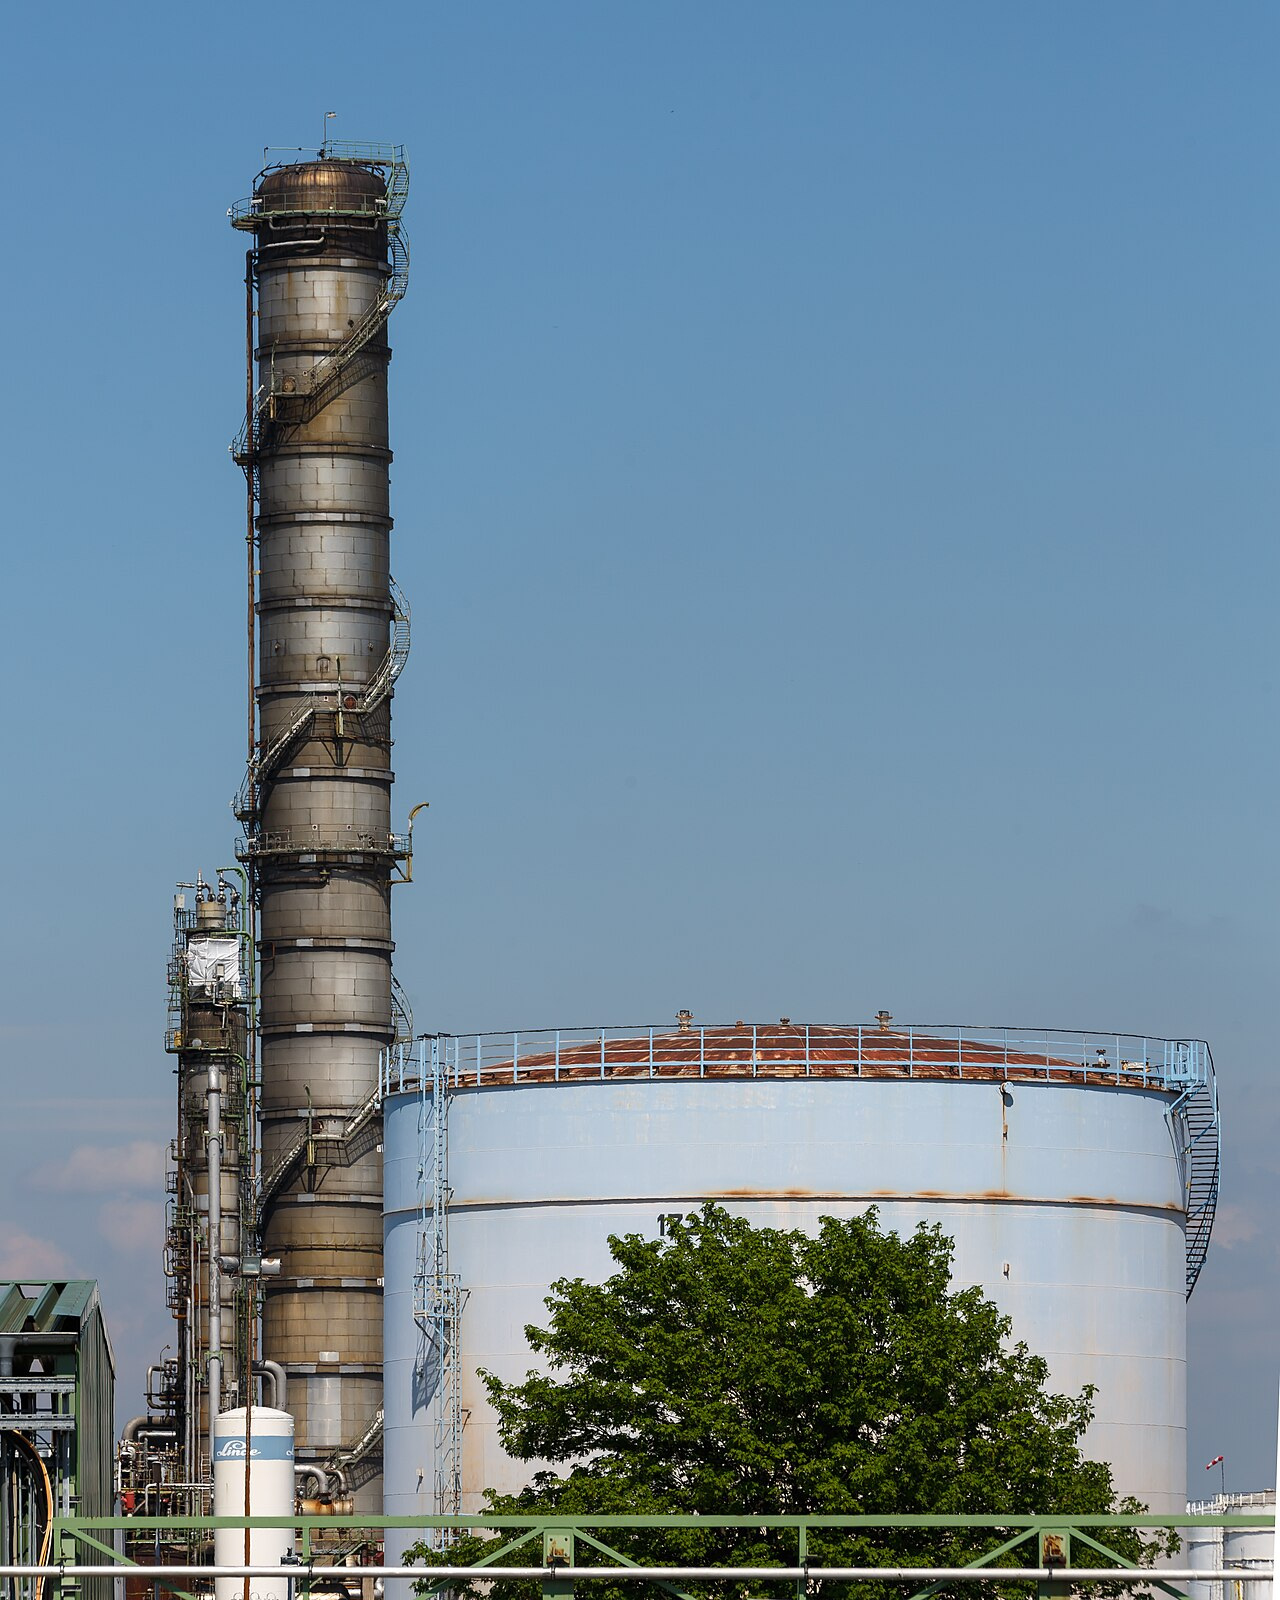
\includegraphics[width=\linewidth]{images/book3/refinery-column.jpg}
\end{minipage}

{\small Kiri: kolom pelat. Cairan mengalir melintasi setiap pelat dan
turun melalui pipa limpah ke pelat di bawahnya; uap naik melalui
pelat-pelat dan menggelegak melewati cairan. Uap yang diembunkan sebagian
dikembalikan sebagai refluks; pendidih ulang di dasar menyediakan uap.
Kanan: kolom distilasi sebuah kilang (Köln, 2014), yang memuat puluhan
pelat. (Foto: CEphoto, Uwe Aranas, CC BY-SA 3.0, Wikimedia Commons.)}
\end{omfigure}

\begin{proposition}[Persamaan Fenske]\label{prop:b2:liquid-vapour-diagrams:fenske}
Pada refluks total, dengan volatilitas relatif $\alpha$ yang tetap, jumlah
\omterm{def:b2:liquid-vapour-diagrams:fractional-distillation}{pelat teoretis} yang diperlukan untuk beralih dari cairan dasar $x_B$ ke
distilat $x_D$ paling sedikit
\[
  N_{\min} = \frac{1}{\ln\alpha}\,\ln\!\left[\frac{x_D}{1 - x_D}\cdot\frac{1 - x_B}{x_B}\right] .
\]
\end{proposition}

\begin{proof}
Beri nomor pelat-pelat itu dari bawah, dengan pendidih ulang sebagai pelat
1. Pada refluks total, cairan yang turun ke pelat $k + 1$ mempunyai
komposisi uap yang meninggalkan pelat $k$: $x_{k+1} = y_k$. Dengan
$r = x/(1 - x)$, setiap pelat memberikan $r(y_k) = \alpha\,r(x_k)$,
sehingga $r(x_{k+1}) = \alpha\,r(x_k)$, dan setelah $N$ pelat uap yang
diembunkan mempunyai $r(x_D) = \alpha^N r(x_B)$. Dengan mengambil
logaritma diperoleh $N$. Dengan refluks berhingga, cairan yang mengalir
turun lebih miskin daripada uap yang naik, setiap pelat memperkaya lebih
sedikit, dan diperlukan lebih banyak pelat.
\end{proof}

Pada diagram $(x, y)$, konstruksi yang sama berupa tangga di antara kurva
kesetimbangan dan diagonal $y = x$: setiap anak tangga adalah satu \omterm{def:b2:liquid-vapour-diagrams:fractional-distillation}{pelat
teoretis}.

\begin{omfigure}
\begin{tikzpicture}
\begin{axis}[width=0.55\linewidth, height=0.55\linewidth, xmin=0, xmax=1,
  ymin=0, ymax=1, axis x line=bottom, axis y line=left,
  xlabel={$x$ (benzena, cair)}, ylabel={$y$ (benzena, uap)},
  tick label style={font=\small}, label style={font=\small}]
\addplot[omThm, thick] table[x=x, y=y] {figdata/out/bachelor-2-liquid-vapour-f-eq.dat};
\addplot[black!50] coordinates {(0,0) (1,1)};
\addplot[omDef, thick] table[x=x, y=y] {figdata/out/bachelor-2-liquid-vapour-f.dat};
\draw[densely dotted] (axis cs:0.95,0) -- (axis cs:0.95,0.95);
\draw[densely dotted] (axis cs:0.05,0) -- (axis cs:0.05,0.05);
\node[font=\scriptsize, anchor=south east] at (axis cs:0.945,0.02) {$x_D$};
\node[font=\scriptsize, anchor=south west] at (axis cs:0.05,0.02) {$x_B$};
\end{axis}
\end{tikzpicture}

{\small Pelat-pelat pada refluks total untuk benzena--toluena, mulai dari
distilat 0.95 ke bawah: setiap langkah mendatar berjalan dari uap ke
cairan yang berada dalam kesetimbangan dengannya (satu pelat), setiap
langkah tegak dari cairan itu ke uap pelat di bawahnya. Tujuh anak tangga
membawa cairan ke bawah $x_B = 0.05$; rumus Fenske memberikan 6.5.}
% ledger: antoine:benzene.A, antoine:toluene.A (computed in figdata/bachelor-2/liquid-vapour.py)
\end{omfigure}

\begin{proposition}[Kolom tidak dapat melintasi azeotrop]\label{prop:b2:liquid-vapour-diagrams:azeotrope-limit}
Dalam campuran yang mempunyai \omterm{def:b2:liquid-vapour-diagrams:azeotrope}{azeotrop}, kolom yang diumpani di salah satu
sisi komposisi \omterm{def:b2:liquid-vapour-diagrams:azeotrope}{azeotrop} paling banyak menghasilkan \omterm{def:b2:liquid-vapour-diagrams:azeotrope}{azeotrop} di satu ujung
dan komponen murni dari sisi itu di ujung yang lain.
\end{proposition}

\begin{proof}
Pada \omterm{def:b2:liquid-vapour-diagrams:azeotrope}{azeotrop}, kurva kesetimbangan bertemu dengan diagonal: $y = x$. Di
dekatnya, setiap anak tangga menjadi sangat kecil, sehingga tidak ada
jumlah pelat berhingga yang mencapainya, dan tidak ada yang melintasinya.
\end{proof}

\begin{method}[Meramalkan distilasi fraksional]\label{met:b2:liquid-vapour-diagrams:predict-distillation}
\begin{enumerate}
  \item Carilah titik didih terendah yang dapat dicapai dari umpan pada
        \omterm{def:b2:liquid-vapour-diagrams:binary-diagram}{diagram isobarik}: komponen murni atau \omterm{def:b2:liquid-vapour-diagrams:azeotrope}{azeotrop positif}. Titik itu
        keluar di puncak.
  \item Titik didih tertinggi di sisi yang sama (komponen murni atau
        \omterm{def:b2:liquid-vapour-diagrams:azeotrope}{azeotrop negatif}) tertinggal di dalam pendidih.
  \item Jika ada \omterm{def:b2:liquid-vapour-diagrams:azeotrope}{azeotrop}, lihatlah di sisi mana umpan berada: hanya
        komponen murni dari sisi itu yang dapat diperoleh.
  \item Untuk jumlah pelat, gunakan rumus Fenske atau tangga itu, lalu
        tambahkan pelat untuk refluks berhingga yang sebenarnya dipakai.
\end{enumerate}
\end{method}

Untuk etanol dan air yang diumpankan pada fraksi kurang dari 0.881, puncak
paling banyak menghasilkan \omterm{def:b2:liquid-vapour-diagrams:azeotrope}{azeotrop} dan dasar menghasilkan air: tidak ada
kolom yang memberikan etanol absolut. Mengeringkan persen terakhir
memerlukan metode lain --- saringan molekul yang mengadsorpsi air, atau
komponen ketiga yang ditambahkan untuk memecah \omterm{def:b2:liquid-vapour-diagrams:azeotrope}{azeotrop}.

\begin{omfigure}
\begin{tikzpicture}[font=\small, scale=0.95, >={Stealth}]
  \pic[transform shape] at (0,0) {heatingmantle};
  \pic[transform shape] at (0,0) {rbflask={0.45}{orange!25}};
  \foreach \x/\y in {-0.35/0.25,0.05/0.18,0.35/0.3}
    \fill[black!55] (\x,\y) circle (0.06);
  % Vigreux column from the flask neck (0,3) to (0,6)
  \draw[om glass] (-0.22,3.0) -- (-0.22,6.0) (0.22,3.0) -- (0.22,6.0);
  \foreach \yy in {3.4,3.9,4.4,4.9,5.4} {
    \draw[om glass] (-0.22,\yy) -- (-0.06,\yy+0.18) -- (-0.22,\yy+0.3);
    \draw[om glass] (0.22,\yy+0.15) -- (0.06,\yy+0.33) -- (0.22,\yy+0.45);
  }
  \pic[transform shape] (s) at (0,6.0) {stillhead};
  \pic[transform shape] at ($(s-top)+(0,-0.75)$) {thermometer};
  \pic[transform shape, rotate=-20] (c) at (s-arm) {liebig={3.4}};
  % ground-glass joint between the head's side arm and the condenser
  \draw[om glass, fill=white, rotate around={-20:(s-arm)}] ($(s-arm)+(-0.12,-0.17)$) rectangle ($(s-arm)+(0.14,0.17)$);
  \coordinate (cend) at ($(s-arm)+(-20:3.4)$);
  \pic[transform shape] (a) at (cend) {adapter};
  \pic[transform shape] at ($(a-tip)+(0,-2.4)$) {erlenmeyer={0.22}{orange!12}};
  \draw[<-, omProp, thick] (-0.25,4.6) -- (-1.6,4.6) node[left, text=black,
    align=right] {kolom Vigreux\\ (lekukan-lekukannya\\ melipatgandakan kontak)};
  \draw[<-, omProp, thick] (0.12,6.72) -- (-1.4,7.4) node[left, text=black,
    align=right] {bola termometer\\ sejajar dengan lengan samping};
  \draw[<-, omProp, thick] (1.08,0.3) -- (2.3,-0.2) node[right, text=black]
    {mantel pemanas};
  \draw[<-, omProp, thick] ($(a-tip)+(0.75,-2.0)$) -- ++(1.0,0.2)
    node[right, text=black] {distilat};
\end{tikzpicture}

{\small \omterm{def:b2:liquid-vapour-diagrams:fractional-distillation}{Distilasi fraksional} di laboratorium. Kolom Vigreux di antara labu
dan kepala distilasi berperan sebagai beberapa \omterm{def:b2:liquid-vapour-diagrams:fractional-distillation}{pelat teoretis}: uap
mengembun pada lekukan-lekukannya dan menguap kembali dalam perjalanannya
naik. Suhu di kepala tetap pada titik didih komponen yang paling mudah
menguap selama komponen itu terdistilasi, lalu naik.}
\end{omfigure}

\begin{inthelab}[Memisahkan dua cairan dengan distilasi fraksional]
Labu diisi paling banyak setengahnya, dengan batu didih, dan dipanaskan
perlahan sehingga cincin uap yang mengembun naik di kolom dengan lambat:
kolom yang terbanjiri karena pemanasan yang cepat kehilangan pelat-pelatnya.
Suhu di kepala dicatat setiap beberapa mililiter; penampung diganti ketika
suhu mulai naik (sebuah \textit{fraksi} dikumpulkan pada setiap anak
tangga suhu), dan pemanasan dihentikan sebelum labu menjadi kering.
\end{inthelab}

\section{Cairan yang sebagian dapat bercampur dan yang tidak dapat bercampur}

\begin{definition}[Celah ketercampuran]\label{def:b2:liquid-vapour-diagrams:miscibility-gap}
Yang disebut \emph{celah ketercampuran}\index{celah ketercampuran} adalah
rentang komposisi keseluruhan tempat dua cairan, pada suhu tertentu,
terpisah menjadi dua lapisan cair, yang masing-masing jenuh dengan komponen
yang lain. Yang disebut \emph{heteroazeotrop}\index{heteroazeotrop} adalah
titik didih cairan dua lapisan semacam itu: kedua lapisan cair dan uap
berdampingan pada suhu tertentu dan dengan komposisi uap tertentu.
\end{definition}

Pada \omterm{def:b2:liquid-vapour-diagrams:miscibility-gap}{heteroazeotrop}, dua komponen berada dalam tiga fase: pada tekanan
tetap \omterm{def:b2:equilibrium-shifts:variance}{variansnya} $2 + 2 - 3 - 1 = 0$. Suhunya tetap, seperti pada titik
didih cairan murni, selama kedua lapisan masih ada.

\begin{omfigure}
\begin{tikzpicture}[font=\small, x=6cm, y=0.08cm]
  \draw[->] (0,0) -- (1.05,0) node[right] {$x$};
  \draw[->] (0,0) -- (0,62) node[above] {$T$};
  \node[below] at (0,0) {2}; \node[below] at (1,0) {1};
  % boiling points: 2 at 50, 1 at 42; heteroazeotrope at 25 with layers 0.1 and 0.85, vapour 0.6
  \draw[omliquidus] (0,50) .. controls (0.04,38) and (0.08,30) .. (0.1,25);
  \draw[omliquidus] (1,42) .. controls (0.95,34) and (0.9,28) .. (0.85,25);
  \draw[omsolidus] (0,50) .. controls (0.25,46) and (0.5,35) .. (0.6,25);
  \draw[omsolidus] (1,42) .. controls (0.9,37) and (0.7,30) .. (0.6,25);
  \draw[thick] (0.1,25) -- (0.85,25);
  \draw[omliquidus] (0.1,25) -- (0.07,2);
  \draw[omliquidus] (0.85,25) -- (0.9,2);
  \fill (0.6,25) circle[radius=2pt];
  \node[font=\scriptsize] at (0.47,6) {dua lapisan cair};
  \node[font=\scriptsize] at (0.5,55) {uap};
  \node[font=\scriptsize] at (0.035,12) {L$_2$};
  \node[font=\scriptsize] at (0.96,12) {L$_1$};
  \node[font=\scriptsize, align=center] at (0.3,33) {L$_2$ + V};
  \node[font=\scriptsize, anchor=west] at (1.06,36) {L$_1$ + V};
  \draw[thin] (1.06,36) -- (0.86,29.5);
  \node[font=\scriptsize, anchor=north] at (0.6,24) {heteroazeotrop};
\end{tikzpicture}

{\small \omterm{def:b2:liquid-vapour-diagrams:binary-diagram}{Diagram isobarik} skematis dua cairan yang sebagian dapat
bercampur. Di bawah suhu \omterm{def:b2:liquid-vapour-diagrams:miscibility-gap}{heteroazeotrop}, cairan terpisah menjadi dua
lapisan L$_1$ dan L$_2$ pada rentang komposisi yang lebar (\omterm{def:b2:liquid-vapour-diagrams:miscibility-gap}{celah
ketercampuran}); pada garis mendatar, kedua lapisan mendidih bersama
menghasilkan uap dengan komposisi tertentu (titik).}
\end{omfigure}

\begin{definition}[Distilasi uap]\label{def:b2:liquid-vapour-diagrams:steam-distillation}
Yang disebut \emph{distilasi uap}\index{distilasi uap} adalah distilasi
cairan yang tidak dapat bercampur dengan air dengan meniupkan uap air ke
dalamnya: campuran itu mendidih di bawah titik didih kedua cairan, dan
distilatnya terpisah menjadi dua lapisan.
\end{definition}

\omterm{def:b2:liquid-vapour-diagrams:steam-distillation}{Distilasi uap} berbeda dari hidrodistilasi pada jilid sekolah hanya dalam
cara memasukkan airnya: uap air ditiupkan melewati bahan, alih-alih bahan
dididihkan di dalam air. Termodinamikanya sama.

\begin{proposition}[Pendidihan dua cairan yang tidak dapat bercampur]\label{prop:b2:liquid-vapour-diagrams:steam}
Dua cairan yang tidak dapat bercampur dan saling bersentuhan mendidih pada
suhu tempat jumlah tekanan uapnya sama dengan tekanan luar,
$p_1^*(T) + p_2^*(T) =
p$, yang lebih rendah daripada kedua titik didih.
Distilatnya mengandung kedua cairan dengan rasio massa
\[
  \frac{m_1}{m_2} = \frac{p_1^*\,M_1}{p_2^*\,M_2} .
\]
\end{proposition}

\begin{proof}
Setiap cairan murni memberikan tekanan uapnya sendiri, berapa pun jumlah
cairan yang lain: tekanan total di atas kedua lapisan adalah
$p_1^* + p_2^*$, yang mencapai $p$ pada suhu tempat setiap $p_i^*$ lebih
kecil daripada $p$. Dalam uap, jumlah zatnya sebanding dengan tekanan
parsialnya, $n_1/n_2 =
p_1^*/p_2^*$; kalikan dengan $M_1/M_2$.
\end{proof}

\begin{omfigure}
\begin{tikzpicture}
\begin{axis}[width=0.6\linewidth, height=5.5cm, xmin=70, xmax=100, ymin=0, ymax=1.6,
  axis x line=bottom, axis y line=left, xlabel={$T$ (\unit{\degreeCelsius})},
  ylabel={$p$ (\unit{bar})}, tick label style={font=\small},
  label style={font=\small}, clip=false]
\addplot[omProp, thick] table[x=t, y=ptol] {figdata/out/bachelor-2-liquid-vapour-e.dat};
\addplot[omDef, thick] table[x=t, y=pwat] {figdata/out/bachelor-2-liquid-vapour-e.dat};
\addplot[black, very thick] table[x=t, y=psum] {figdata/out/bachelor-2-liquid-vapour-e.dat};
\draw[densely dashed] (axis cs:70,1.013) -- (axis cs:100,1.013) node[right, font=\scriptsize] {\qty{1.013}{bar}};
\draw[densely dotted] (axis cs:84.3,0) -- (axis cs:84.3,1.013);
\node[font=\scriptsize, anchor=south east] at (axis cs:84.3,1.05) {\qty{84.3}{\degreeCelsius}};
\node[font=\scriptsize, anchor=west] at (axis cs:96,1.45) {jumlah};
\node[font=\scriptsize, omDef, anchor=south] at (axis cs:77,0.46) {air};
\node[font=\scriptsize, omProp, anchor=north west] at (axis cs:88,0.5) {toluena};
\end{axis}
\end{tikzpicture}

{\small Toluena dan air, yang tidak dapat bercampur: tekanan uap
masing-masing cairan dan jumlahnya. Kedua lapisan mendidih bersama pada
\qty{84.3}{\degreeCelsius}, di bawah titik didih air (\qty{100}{\degreeCelsius})
dan toluena (\qty{110.6}{\degreeCelsius}); distilatnya membawa 4.1 g
toluena per gram air.}
% ledger: antoine:toluene.A, antoine:water.A, aw:C, aw:H, aw:O (computed in figdata/bachelor-2/liquid-vapour.py)
\end{omfigure}

Molekul-molekul esens tumbuhan yang berat dan rapuh terdistilasi dengan
cara ini pada suhu sedikit di bawah \qty{100}{\degreeCelsius}, jauh di
bawah titik didihnya sendiri, dengan sedikit dekomposisi; harganya adalah
distilat yang sebagian besar berupa air.

\section{Latihan}

\begin{exercise}[$\star$]\label{exo:b2:liquid-vapour-diagrams:1}
Pada \omterm{def:b2:liquid-vapour-diagrams:binary-diagram}{diagram isobarik} benzena--toluena, bacalah titik didih kedua cairan
murni, \omterm{def:b2:liquid-vapour-diagrams:bubble-dew}{titik gelembung} cairan dengan komposisi 0.2, dan komposisi uap
pertamanya.
\end{exercise}

\begin{exercise}[$\star$]\label{exo:b2:liquid-vapour-diagrams:2}
Pada \qty{80}{\degreeCelsius}, tekanan uap benzena dan toluena adalah
\qty{1.010}{bar} dan \qty{0.388}{bar}. Hitunglah, untuk cairan ekuimolar,
tekanan saat cairan itu mulai mendidih dan komposisi uapnya.
\end{exercise}

\begin{exercise}[$\star$]\label{exo:b2:liquid-vapour-diagrams:3}
Sebanyak \qty{10}{mol} campuran dengan komposisi keseluruhan 0.30 berada
pada suhu tempat cairannya berkomposisi 0.20 dan uapnya 0.45. Hitunglah
jumlah zat setiap fase.
\end{exercise}

\begin{exercise}[$\star$]\label{exo:b2:liquid-vapour-diagrams:4}
Hitunglah \omterm{def:b2:equilibrium-shifts:variance}{varians} campuran benzena--toluena (a) yang seluruhnya cair;
(b) yang sedang mendidih; (c) pada \omterm{def:b2:liquid-vapour-diagrams:azeotrope}{azeotrop}, untuk pasangan yang
mempunyainya, pada tekanan tetap.
\end{exercise}

\begin{exercise}[$\star\star$]\label{exo:b2:liquid-vapour-diagrams:5}
Tentukan dengan coba-coba \omterm{def:b2:liquid-vapour-diagrams:bubble-dew}{titik embun} uap benzena--toluena berkomposisi
0.30 pada \qty{1.013}{bar}, dengan $p^*_{\text{benzena}}$ dan
$p^*_{\text{toluena}}$ (\unit{bar}): 1.80 dan 0.742 pada
\qty{100}{\degreeCelsius}, 2.057 dan 0.861 pada \qty{105}{\degreeCelsius}.
Berikan komposisi tetes pertamanya.
\end{exercise}

\begin{exercise}[$\star\star$]\label{exo:b2:liquid-vapour-diagrams:6}
Campuran ekuimolar benzena--toluena didistilasi secara sederhana (tanpa
kolom). Berapa komposisi tetes-tetes distilat pertama? Bagaimana suhu dan
komposisi distilat berubah selama distilasi berlangsung? Mengapa
pemisahannya buruk?
\end{exercise}

\begin{exercise}[$\star\star$]\label{exo:b2:liquid-vapour-diagrams:7}
Anggur dengan fraksi mol etanol 0.05 didistilasi secara fraksional dengan
kolom yang sangat efisien. Apa yang keluar di puncak, dan apa yang
tertinggal di dalam pendidih? Pertanyaan yang sama untuk campuran dengan
fraksi mol 0.95.
\end{exercise}

\begin{exercise}[$\star\star$]\label{exo:b2:liquid-vapour-diagrams:8}
Sebuah komponen esens tumbuhan (massa molar \qty{136}{g/mol}) mempunyai
tekanan uap \qty{0.10}{bar} di dekat \qty{97}{\degreeCelsius}, ketika
tekanan uap air \qty{0.91}{bar} (data latihan). Pada suhu berapa \omterm{def:b2:liquid-vapour-diagrams:steam-distillation}{distilasi
uap} berlangsung di bawah \qty{1.013}{bar}, dan berapa gram esens yang
dikumpulkan per gram air?
\end{exercise}

\begin{exercise}[$\star\star$]\label{exo:b2:liquid-vapour-diagrams:9}
Pada diagram skematis cairan yang sebagian dapat bercampur, uraikan apa
yang terjadi jika campuran dua lapisan dengan komposisi keseluruhan 0.4
dipanaskan dari suhu kamar sampai seluruhnya menjadi uap: fase-fasenya,
suhu-suhunya, dan komposisi uap pertamanya.
\end{exercise}

\begin{exercise}[$\star\star\star$]\label{exo:b2:liquid-vapour-diagrams:10}
Dengan $\alpha = 2.47$, hitunglah jumlah minimum \omterm{def:b2:liquid-vapour-diagrams:fractional-distillation}{pelat teoretis} untuk
distilat 0.99 dan dasar 0.01. Bandingkan dengan 6.5 yang diperlukan untuk
0.95 dan 0.05, lalu berilah komentar tentang harga kemurnian.
\end{exercise}

\begin{exercise}[$\star\star\star$]\label{exo:b2:liquid-vapour-diagrams:11}
Dari \omterm{def:b2:liquid-vapour-diagrams:binary-diagram}{diagram isobarik} benzena--toluena dan persamaan Antoine, jelaskan
bagaimana \omterm{def:b2:liquid-vapour-diagrams:binary-diagram}{diagram isotermal} pada \qty{80}{\degreeCelsius} diperoleh, dan
mengapa pada diagram itu daerah cair berada di atas.
\end{exercise}

\begin{exercise}[$\star\star\star$]\label{exo:b2:liquid-vapour-diagrams:12}
Mulai dari hubungan $d\ln p = (y - x)\,dy/[y(1 - y)]$, tunjukkan bahwa pada
suhu tetap tekanan total bertambah seiring $x$ di mana pun uap lebih kaya
akan komponen 1 daripada cairannya, lalu simpulkan bahwa \omterm{def:b2:chemical-potential:ideal-mixture}{campuran ideal}
tidak mempunyai \omterm{def:b2:liquid-vapour-diagrams:azeotrope}{azeotrop}.
\end{exercise}

\section{Soal: Sebuah Kolom untuk Benzena dan Toluena}

\begin{problem}[{Soal akhir pekan --- diagram isobarik benzena dan toluena
dari persamaan Antoine, penguapan kilat dan aturan tuas, jumlah minimum
pelat kolom pada refluks total, dan batas yang ditetapkan oleh azeotrop}]
\label{pb:b2:liquid-vapour-diagrams:1}
Data: persamaan Antoine, $\log_{10}(p^*/\unit{bar}) = A - B/(T + C)$ dengan
$T$ dalam kelvin: benzena $A = 4.01814$, $B = \qty{1203.835}{K}$, $C =
\qty{-53.226}{K}$; toluena $A = 4.07827$, $B = \qty{1343.943}{K}$, $C =
\qty{-53.773}{K}$. Tekanan \qty{1.013}{bar}; benzena dan toluena
membentuk \omterm{def:b2:chemical-potential:ideal-mixture}{campuran ideal}. \omterm{def:b2:liquid-vapour-diagrams:azeotrope}{Azeotrop} etanol--air mengandung 95~\% massa
etanol.
% ledger: antoine:benzene.A, antoine:benzene.B, antoine:benzene.C, antoine:toluene.A, antoine:toluene.B, antoine:toluene.C, azeo:ethanol-water.w

\medskip
\noindent\textbf{Bagian I --- Diagram.}
\begin{enumerate}
  \item Hitunglah titik didih benzena dan toluena pada \qty{1.013}{bar}.
  \item Hitunglah $p_1^*$ dan $p_2^*$ pada \qty{90}{\degreeCelsius}.
  \item Simpulkan komposisi cairan dan uap yang berada dalam
        kesetimbangan pada \qty{90}{\degreeCelsius}.
  \item Hal yang sama pada \qty{100}{\degreeCelsius} ($p_1^* = \qty{1.800}{bar}$,
        $p_2^* =
        \qty{0.742}{bar}$).
  \item Sketsalah \omterm{def:b2:liquid-vapour-diagrams:binary-diagram}{diagram isobarik} dari keempat titik ini dan cairan-cairan
        murninya.
  \item Tentukan \omterm{def:b2:liquid-vapour-diagrams:bubble-dew}{titik gelembung} cairan ekuimolar, dengan ketelitian
        \qty{0.5}{\degreeCelsius}, dengan coba-coba antara
        \qty{90}{\degreeCelsius} dan \qty{95}{\degreeCelsius}.
  \item Hitunglah \omterm{def:b2:equilibrium-shifts:variance}{varians} campuran yang mendidih dan nyatakan apa artinya
        bagi diagram.
\end{enumerate}

\medskip
\noindent\textbf{Bagian II --- Penguapan kilat.}
\begin{enumerate}[resume]
  \item Umpan ekuimolar dipanaskan sampai \qty{95}{\degreeCelsius}
        ($p_1^* =
        \qty{1.569}{bar}$, $p_2^* = \qty{0.636}{bar}$). Hitunglah
        $x$ dan $y$.
  \item Untuk \qty{100}{mol} umpan, hitunglah jumlah cairan dan uap.
  \item Hitunglah jumlah benzena dalam setiap fase dan periksalah
        neracanya.
  \item Berapa bagian benzena yang diperoleh kembali di dalam uap?
  \item Apa yang terjadi jika penguapan kilat dijalankan pada
        \qty{100}{\degreeCelsius}?
  \item Pada suhu berapa umpan itu seluruhnya teruapkan?
\end{enumerate}

\medskip
\noindent\textbf{Bagian III --- Kolom.}
\begin{enumerate}[resume]
  \item Definisikan volatilitas relatif $\alpha$ dan hitunglah nilainya
        pada titik didih benzena.
  \item Hitunglah nilainya pada titik didih toluena.
  \item Ambillah rata-rata geometrisnya sebagai nilai untuk seluruh kolom.
  \item Tunjukkan bahwa pada \omterm{def:b2:liquid-vapour-diagrams:fractional-distillation}{pelat teoretis} $y/(1 - y) = \alpha\,x/(1 - x)$.
  \item Jelaskan mengapa, pada refluks total, cairan yang masuk ke sebuah
        pelat mempunyai komposisi uap yang meninggalkan pelat di bawahnya.
  \item Turunkan rumus Fenske.
  \item Hitunglah jumlah minimum \omterm{def:b2:liquid-vapour-diagrams:fractional-distillation}{pelat teoretis} untuk distilat 0.95 dan
        dasar 0.05.
  \item Mengapa kolom nyata diberi lebih banyak pelat daripada itu?
  \item Pada tangga dalam bab ini, hitunglah anak tangganya lalu
        bandingkan.
\end{enumerate}

\medskip
\noindent\textbf{Bagian IV --- Sebuah \omterm{def:b2:liquid-vapour-diagrams:azeotrope}{azeotrop}.}
\begin{enumerate}[resume]
  \item Hitunglah fraksi mol etanol dalam \omterm{def:b2:liquid-vapour-diagrams:azeotrope}{azeotrop} etanol--air.
  \item Umpan etanol 0.10 masuk ke kolom dengan lima puluh pelat. Apa yang
        keluar di puncak dan di dasar?
  \item Nyatakan jumlah minimum \omterm{def:b2:liquid-vapour-diagrams:fractional-distillation}{pelat teoretis} yang diperlukan untuk
        memisahkan benzena dan toluena menjadi produk-produk 95~\%.
\end{enumerate}
\end{problem}
